\chapter{Preliminary Work}
\label{chap:prelim_work}
Several steps are necessary to accomplish the objectives of this research.

%--------------------------------------------------------------------------------------------------------------------------------------------------------------------
%--------------------------------------------------------------------------------------------------------------------------------------------------------------------
%--------------------------------------------------------------------------------------------------------------------------------------------------------------------
%--------------------------------------------------------------------------------------------------------------------------------------------------------------------
%--------------------------------------------------------------------------------------------------------------------------------------------------------------------
%--------------------------------------------------------------------------------------------------------------------------------------------------------------------
%--------------------------------------------------------------------------------------------------------------------------------------------------------------------
\section{Nonlinear \cobra}
\label{sect:nl_cobra}
The first stage of preliminary work was to modify the \cobra software.
The \cobra software as obtained was a single-shot linearization version of the semi-implicit method.
In order to evaluate the spatially-selective nonlinear refinement idea, \cobra needed to be able to solve nonlinear problems.
\cobra needed to be converted to a fully iterative nonlinear solver.
When it is necessary to distinguish between the single-shot linearization algorithmic implementation of \cobra and the iterative nonlinear \cobra, the former shall be referred to as legacy mode and the latter as nonlinear mode.
As such, the objectives of this work were to modify the software to be able do the following:

\begin{itemize}
\item{Create a data framework for constructing vector quantities such as $\vec{x}^{k}$ and $\vec{F}$.}
\item{Correctly evaluate $\vec{F}(\vec{x}^{k})$ and $\vec{J}(x^{k})$.}
\item{Implement a globalization strategy for Newton's method.}
\end{itemize}

\cobra utilized a single-shot linearization newton method for its solution technique.
As a result of that design decision, certain memory savings techniques were employed in its construction that precluded the idea of more than one Newton step.
In particular, there was an implicit assumption within the software that the current Newton iterate, $\vec{x}^{n+1, 0}$, was the old-time variable $\vec{x}^{n}$.
This design decision required an an evaluation of all routine involved with the evaluation of components of both the nonlinear residual and the Jacobian.
In addition, the assumption that $\vec{x}^{n+1, k} = \vec{x}^{n}$ required identification of places in the source code where there were implicit cancellation of terms.
Where appropriate, the software was changed to reflect the distinction between old-time and iterate variables and to introduce terms that had been assumed to be equal to zero.

Once the appropriate variables were used for the evaluation of nonlinear residuals and Jacobians, a Newton loop was introduced to allow multiple Newton steps.
\alg{alg:nl_cobra} contains the current algorithmic implementation of the non-linear semi-implicit method.

\begin{algo}[H]
\caption{Nonlinear \cobra solution algorithm.}
\label{alg:nl_cobra}
\setlength{\baselineskip}{0.625\baselineskip}
\begin{algorithmic}[1]
\Require $\vec{x}^{0}$ and $t^{0}$
\Set $n = 0$
\Loop \; Transient Loop
    \State $t^{n+1} : = t^{n} + \Delta t$
    \State $k = 0$
    \State $\vec{x}^{n+1,0} = \vec{x}^{n}$
	\Calculate $\vec{F}(\vec{x}^{n+1,0})$ and $\vec{J}(\vec{x}^{n+1,0})$
    \Loop \; Newton Loop
		\Calculate $\vec{\delta x} = - \vec{J}^{-1}\cdot\vec{F}$
		$j = 0$		
		\Calculate $\vec{x}^{n+1,k+1,j}$
		\Calculate $\vec{F}(\vec{x}^{n+1,k+1,j})$
		\Loop \; Globalization Loop
			\If{ Globalization loop termination criteria not met}
				\Calculate $\lambda_j$
				\Calculate $\vec{x}^{n+1,k+1,j+1} = \vec{x}^{n+1,k} + \lambda \vec{\delta x}$
				\Calculate $\vec{F}(\vec{x}^{n+1,k+1,j+1})$
				\State $j = j + 1$			
			\Else
				\Calculate $\vec{J}(\vec{x}^{n+1,k+1,j})$
				\Exit Globalization Loop
			\EndIf
		\EndLoop			
		\If{ Newton loop termination criteria met}
			\Exit Newton Loop
		\EndIf
	\EndLoop
	\State $n = n + 1$
\EndLoop
\end{algorithmic}
\end{algo}

In \alg{alg:nl_cobra}, there are three steps that require discussion.
First is the Newton Loop termination criteria.
There are three Newton loop termination mechanisms, listed below.

\begin{itemize}
\item{Maximum number of Newton iterates, $k_{\,\text{MAX}}$, exceeded.}
\item{The L-inf norm of the scaled residual, $||\vec{S}^{-1}\vec{F}||_{\infty}$, is below a specified threshold, $F_{\text{ABS}}$.}
\item{The L-inf norm of the scaled update, $||\vec{D}^{-1}\vec{\delta x}||_{\infty}$, is below a specified threshold, $\delta_{\text{ABS}}$.}
\end{itemize}

Current values for $k_{\,\text{MAX}}$, $F_{\text{ABS}}$ and $\delta_{\text{ABS}}$ are $35$, $1.0$E$-05$, and $1.0$E$-10$, respectively.
The scaling vectors, $\vec{S}$ and $\vec{D}$, will be addressed later.

The globalization strategy implemented in \cobra is a linesearch algorithm \cite{Dennis1996}.
The two globalization loop termination criteria are listed below.
\begin{itemize}
\item{$\frac{1}{2}||\vec{F}^{k+1, j}||_{2} < \frac{1}{2}||\vec{F}^{k}||_{2} - \alpha ||\vec{F}^{k}||_{2}$ }
\item{$||\lambda_{j+1} \vec{\delta x}||_{\infty} < \delta_{\text{abs}}$}
\end{itemize}

If neither of the loop termination criteria are met, then the a step-length parameter, $\lambda_j$ is calculated.
On the first pass through the globalization loop within a given Newton step, a quadratic backtracking model is adopted.
On subsequent passes, a cubic-backtracking model is used.
 
Since vector forms of the nonlinear residual and the independent parameters are used in determining nonlinear convergence and in the globalization algorithm, they needed to be easily manipulated.
A subroutine was written to gather the discrete variables of the independent parameters into a single vector.
Additional source code modifications were necessary to construct and gather the components of the nonlinear residual.

%--------------------------------------------------------------------------------------------------------------------------------------------------------------------
%--------------------------------------------------------------------------------------------------------------------------------------------------------------------
%--------------------------------------------------------------------------------------------------------------------------------------------------------------------
%--------------------------------------------------------------------------------------------------------------------------------------------------------------------
%--------------------------------------------------------------------------------------------------------------------------------------------------------------------
%--------------------------------------------------------------------------------------------------------------------------------------------------------------------
%--------------------------------------------------------------------------------------------------------------------------------------------------------------------
\section{Operator Based Scaling}
\label{sect:operator_scaling}
In order to determine the degree to which a state vector, $\vec{x}$, satisfies \eqref{eqn:conservation_equations}, the use of the nonlinear residual, $\vec{F}$, is required.
However, due to the formulation of the residual vector, the magnitudes of residuals can vary by orders of magnitude.
For a given grid location, the nonlinear residuals for mass and energy as formulated in section \ref{subsect:semi_implicit} will have six components.
These residuals will have the units of the conserved quantities for their corresponding PDEs.
Table \ref{tab:scaling_units_scales} shows the range of parameters possible within \cobra.

\begin{table}[ht]
\centering
\begin{tabular}{@{}c@{}} \toprule
Scale \\
\bottomrule  
\end{tabular}
\caption{Typical scale for reactor simulations}
\label{tab:scaling_units_scales}
\end{table}

However, during accident scenarios, the range of these values can dramatically change.
One of the challenges that has been addressed during this work is coming up with a method for scaling that will provide a meaningful metric for convergence.
The scaling chosen should have the following characteristics:
\begin{itemize}
\item{$S^{-1}_k F(x_k)_i \approx 1$ when $x_k$ is a "poor" solution.}
\item{$S^{-1}_k F(x_k)_i \rightarrow 0$ when a phase disappears.}
\item{$0 \leq S^{-1}_k F(x_k)_i \leq 1 $ for all values of $F(x_k)_i$.}
\end{itemize}

The heart of the scaling used in this work is a physics-based method.
To illustrate the scaling procedure, we shall consider \eqref{eqn:conservation_of_liq} for a simply connected continuity cell without inter-field mass transfer.
Assume that the entire channel single phase and in thermodynamics equilibrium such that the macroscopic densities on either side of this single cell are the same.

\begin{equation}
F = \left(\alpha_k \rho_k\right)^{n+1} - \left( \alpha_k \rho_k \right)^n - \frac{\Delta t}{V} \left( \frac{\alpha_k \rho_k }{<\alpha_k \rho_k>^n} V^{n+1}_{j-1} \right)
\end{equation}

In this equation there are three physically meaningful quantities: the temporal difference, the mass flowing into the cell, and mass flowing out of the volume. 

%--------------------------------------------------------------------------------------------------------------------------------------------------------------------
%--------------------------------------------------------------------------------------------------------------------------------------------------------------------
%--------------------------------------------------------------------------------------------------------------------------------------------------------------------
%--------------------------------------------------------------------------------------------------------------------------------------------------------------------
%--------------------------------------------------------------------------------------------------------------------------------------------------------------------
%--------------------------------------------------------------------------------------------------------------------------------------------------------------------
%--------------------------------------------------------------------------------------------------------------------------------------------------------------------
\section{Temporal Convergence}
\label{sect:temporal_convergence}
As stated in \sect{subsect:temporal_approx}, if the nonlinearities of the discrete governing equations are not resolved, then temporal convergence can be degraded.
This degradation can produce results that qualitatively appear to be converged.
This apparent convergence, or time-step size insensitivity, is a result not of reaching a time-step size insensitive solution, but, instead, is indicative of highly degrade order of accuracy due to the failure to resolve the nonlinearities at each time-step.
With the first-order methods outlined in \sect{sect:solution_techniques}, this degradation can result in methods that are approximately zeroth order \cite{Knoll2001}.
To determine if the validity of the transient solution is both time-step size insensitive and an accurate solution to the nonlinear problem, a quantifiable metric is sought.

The scaled residual from \sect{sect:operator_scaling} provides a well-scaled metric for instantaneous nonlinear convergence at any given time in the simulation.
The natural extension of this metric would be a temporal integral of the global nonlinear residual, \eqref{eqn:trans_res_simple}.

\begin{equation}
\label{eqn:trans_res_simple}
\vec{R} = \int_{t^{0}}^{t^{N}} ||\vec{F}(\tau)||_2 \,\mathrm{d} \tau
\end{equation}

Given the bounds of the scaled residual, \eqref{eqn:scaled_residual}, it was considered desirable to have a similarly scaled transient residual.
The transient residual in \eqref{eqn:trans_res_simple} posses a dependence upon the number of time-steps taken.
To remove this dependence, a temporal average was instead investigated, \eqref{eqn:trans_res_ave}.

\begin{equation}
\label{eqn:trans_res_ave}
\vec{R} = \frac{\int_{t^{0}}^{t^{N}} ||\vec{F}(\tau)||_2 \,\mathrm{d} \tau}{t^{N} - t^{0}}
\end{equation}

This metric posses the desirable bound stated above.
Other weighted temporal integrals were considered, such as a simple moment about $t^{0}$, \eqref{eqn:trans_res_mom}.
However, this moment has the the theoretical disadvantage of weighting the latter portion of the transient.

\begin{equation}
\label{eqn:trans_res_mom}
\vec{R} = \frac{\int_{t^{0}}^{t^{N}} \,\tau\,||\vec{F}(\tau)||_2 \,\mathrm{d} \tau}{\int_{t^{0}}^{t^{N}} \,\tau \,\mathrm{d} \tau}
\end{equation}

For the preliminary work, the \eqref{eqn:trans_res_ave} and \eqref{eqn:trans_res_mom} were selected for evaluation.

%--------------------------------------------------------------------------------------------------------------------------------------------------------------------
%--------------------------------------------------------------------------------------------------------------------------------------------------------------------
%--------------------------------------------------------------------------------------------------------------------------------------------------------------------
%--------------------------------------------------------------------------------------------------------------------------------------------------------------------
%--------------------------------------------------------------------------------------------------------------------------------------------------------------------
%--------------------------------------------------------------------------------------------------------------------------------------------------------------------
%--------------------------------------------------------------------------------------------------------------------------------------------------------------------

\section{Numerical Experiments}
\label{sect:numerical_experiments}

Two test problems were constructed to examine the impact of nonlinear convergence on temporal convergence.
The primary objective of these tests is to determine the impact of resolving the nonlinearities at each time step for a given time-step maximum time-step size on the number of time-step size refinements necessary to reach a temporally converged solution.
A secondary objective is an evaluation of the temporal convergence metric.

\subsection{Geometry}
\label{subsect:experimental_geometry}
For both of the test problems, the same computational geometry was used; figure \ref{fig:exp_geometry} represents the experimental geometry.
Each block represents a single continuity cell with a height of 4 [in].
The total height of the channel is 48 [in].
Each continuity cell has a cross-sectional area of 4 [in$^2$] and a hydraulic diameter of 4 [in].
The red block at the top of the channel represents a boundary cell where the pressure and enthalpy are specified.
This boundary represents an infinite reservoir filled with a fluid at a specified thermodynamic state.
The red triangle represents a specified flow at the bottom edge of the first continuity cell. 

\begin{figure}[h!t]
\label{fig:exp_geometry}
\begin{center}
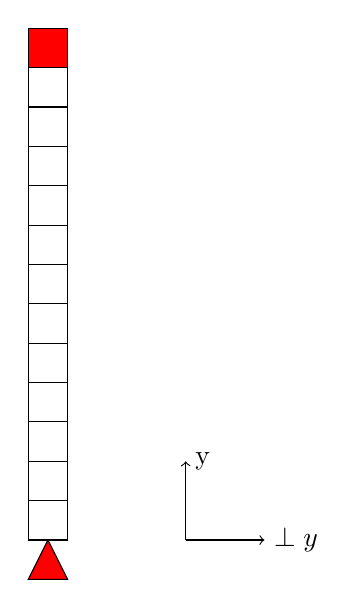
\begin{tikzpicture}
\foreach \x in {1,..., 12} \draw(0, 0.5*\x-0.5) rectangle +(.5,.5);
\filldraw[fill=red] (0, 6) rectangle +(.5,.5); 
\filldraw[fill=red] (0, -0.5) -- (0.25, 0) -- (0.5, -0.5) -- cycle;
\draw[->] (2,0) -- (2, 1) node[anchor=west] {y};
\draw[->] (2,0) -- (3, 0) node[anchor=west] {$\perp y$};
\end{tikzpicture}
\end{center}
\caption{Geometry for test problems.}
\end{figure}

\subsection{Initial and Boundary Conditions}
\label{subsect:ic_bc}

The two problems, while having the same geometry, are different in their dominant physics.
One problem was designed to represent single-phase, single-field continuous liquid flow in a standpipe; this problem will be referred to as the "Single Phase" problem.
The second problem was designed such that high pressure liquid flashes into steam as it enters a standpipe initially filled with saturated vapor at a much lower pressure, known hereafter as the "Flashing" problem.

Table \ref{tab:ic} provides the initial conditions for the two problems.
The pressure, enthalpy, and volume-fractions for the different fields allows for a complete description of the continuity variables.
The initial velocities are set to zero.

\begin{table}[ht]
\centering
\begin{tabular}{@{}lr@{.}lr@{.}lr@{.}lr@{.}lr@{.}l@{}} \toprule
\multirow{2}{*}{Problem} & \multicolumn{2}{c}{Pressure} & \multicolumn{2}{c}{Enthalpy}             & \multicolumn{2}{c}{$\alpha_g$} & \multicolumn{2}{c}{$\alpha_l$} & \multicolumn{2}{c}{$\alpha_e$} \\ 
                         & \multicolumn{2}{c}{[psia]} & \multicolumn{2}{c}{$[\frac{\text{Btu}}{\text{lb}_{\text{m}}}]$} & \multicolumn{2}{c}{[-]}      & \multicolumn{2}{c}{[-]}      & \multicolumn{2}{c}{[-]}      \\ \midrule
Single Phase             &  200&0                       &  355&5                                   & 0&0                            & 1&0                            & 0&0 \\
Flashing                 &  200&0                       & 1198&3                                   & 1&0                            & 0&0                            & 0&0 \\ \bottomrule  
\end{tabular}
\caption{Initial conditions for test problems.}
\label{tab:ic}
\end{table}

Each of the problems has a specified pressure-enthalpy boundary condition at the top of the stand pipe and a flow-enthalpy boundary condition at the inlet of the domain.
Table \ref{tab:bc_pe} contains the pressure, enthalpy, and composition of the pressure-enthalpy reservoir. 

\begin{table}[ht]
\centering
\begin{tabular}{@{}lr@{.}lr@{.}lr@{.}lr@{.}lr@{.}l@{}} \toprule
\multirow{2}{*}{Problem} & \multicolumn{2}{c}{Pressure} & \multicolumn{2}{c}{Enthalpy}             & \multicolumn{2}{c}{$\alpha_g$} & \multicolumn{2}{c}{$\alpha_l$} & \multicolumn{2}{c}{$\alpha_e$} \\ 
                         & \multicolumn{2}{c}{[psia]} & \multicolumn{2}{c}{$[\frac{\text{Btu}}{\text{lb}_{\text{m}}}]$} & \multicolumn{2}{c}{[-]}      & \multicolumn{2}{c}{[-]}      & \multicolumn{2}{c}{[-]}      \\ \midrule
Single Phase             &  200&0                       &  355&5                                   & 0&0                            & 1&0                            & 0&0 \\
Flashing                 &  200&0                       & 1198&3                                   & 1&0                            & 0&0                            & 0&0 \\ \bottomrule  
\end{tabular}
\caption{Pressure-enthalpy boundary conditions for test problems.}
\label{tab:bc_pe}
\end{table}

The flow-enthalpy boundary condition describes the thermodynamic state of the inflowing fluid and the rate at its flowrate.
Table \ref{tab:bc_fe} describes the inlet boundary condition for the two problems.

\begin{table}[ht]
\centering
\begin{tabular}{@{}lr@{.}lr@{.}lr@{.}lr@{.}lr@{.}l@{}} \toprule
\multirow{2}{*}{Problem} & \multicolumn{2}{c}{Pressure} & \multicolumn{2}{c}{Enthalpy}             & \multicolumn{2}{c}{$\alpha_g$} & \multicolumn{2}{c}{$\alpha_l$} & \multicolumn{2}{c}{$\alpha_e$} \\ 
                         & \multicolumn{2}{c}{[psia]} & \multicolumn{2}{c}{$[\frac{\text{Btu}}{\text{lb}_{\text{m}}}]$} & \multicolumn{2}{c}{[-]}      & \multicolumn{2}{c}{[-]}      & \multicolumn{2}{c}{[-]}      \\ \midrule
Single Phase             &  200&0                       &  355&5                                   & 0&0                            & 1&0                            & 0&0 \\
Flashing                 & 1000&0                       &  542&6                                   & 1&0                            & 0&0                            & 0&0 \\ \bottomrule  
\end{tabular}
\caption{Flow-enthalpy boundary conditions for test problems.}
\label{tab:bc_fe}
\end{table}

The specified mass flow, $\dot{m}(t)$, at the bottom of the channels is the same for both problems. 
The is a time-dependent function give by \eqref{eqn:bc_time_func_single}.

\begin{equation}
\label{eqn:bc_time_func_single}
\dot{m}(t) = \left\{
\begin{array}{cclrcll}
 0.0           & [\frac{\text{lb}_{\text{m}}}{\text{s}}] & , &         & t & \leq 1 &[\text{s}] \\
 0.5 ( t - 1)  & [\frac{\text{lb}_{\text{m}}}{\text{s}}] & , & 1 [\text{s}] < & t & \leq 2 &[\text{s}] \\
 0.5           & [\frac{\text{lb}_{\text{m}}}{\text{s}}] & , &         & t & > 2    &[\text{s}]
\end{array}\right.
\end{equation}

Both problems adjust their initial pressure distribution to account for hydrostatic head, which is not specified on the inlet cards.
The \cobra input deck for both problems can be found in \app{app:input_decks}.

\subsection{Procedure}
\label{subsect:experiments_procedure}
The two problems were set up such that the maximum allowable time-step could be varied.
Each problem was run with the following maximum allowable time-steps: 1 [s], 0.1 [s], 0.01 [s], 0.001 [s], 0.0001 [s], and 0.00001 [s]. 
For the legacy runs, the nonlinear residual was evaluated with the result of a single newton-step.
For the nonlinear runs, the nonlinear residuals were evaluated at the end of the newton-loop.
The temporal convergence metric was evaluated during post processing.

\subsection{Results}
\label{subsect:results}
First, the temporal convergence metrics will be discussed.

\begin{table}[h!t]
\centering
\begin{tabular}{@{}l r@{.}l r@{.}l r@{.}l r@{.}l @{}}
\toprule
& \multicolumn{4}{c}{Single Phase} & \multicolumn{4}{c}{Flashing}  \\
$\Delta t_{\text{MAX}}$ & \multicolumn{2}{c}{Legacy} & \multicolumn{2}{c}{Nonlinear} & \multicolumn{2}{c}{Legacy}& \multicolumn{2}{c}{Nonlinear}  \\
\midrule
1.0    & 2&03E-2 & 2&03E-2 & \multicolumn{2}{c}{-} & 2&03E-2 \\
1.0E-1 & 2&03E-2 & 2&03E-2 & 2&03E-2 & 2&03E-2 \\
1.0E-2 & 2&03E-2 & 2&03E-2 & 2&03E-2 & 2&03E-2 \\
1.0E-3 & 2&03E-2 & 2&03E-2 & 2&03E-2 & 2&03E-2 \\
1.0E-4 & 2&03E-2 & 2&03E-2 & 2&03E-2 & 2&03E-2 \\
1.0E-5 & 2&03E-2 & 2&03E-2 & 2&03E-2 & 2&03E-2 \\
\bottomrule  
\end{tabular}
\caption{Temporal convergence metric -- average}
\label{tab:criteria_ave}
\end{table}


\begin{table}[h!t]
\centering
\begin{tabular}{@{}l r@{.}l r@{.}l r@{.}l r@{.}l @{}}
\toprule
& \multicolumn{4}{c}{Single Phase} & \multicolumn{4}{c}{Flashing}  \\
$\Delta t_{\text{MAX}}$ & \multicolumn{2}{c}{Legacy} & \multicolumn{2}{c}{Nonlinear} & \multicolumn{2}{c}{Legacy}& \multicolumn{2}{c}{Nonlinear}  \\
\midrule
1.0    & 2&03E-2 & 2&03E-2 & \multicolumn{2}{c}{-} & 2&03E-2 \\
1.0E-1 & 2&03E-2 & 2&03E-2 & 2&03E-2 & 2&03E-2 \\
1.0E-2 & 2&03E-2 & 2&03E-2 & 2&03E-2 & 2&03E-2 \\
1.0E-3 & 2&03E-2 & 2&03E-2 & 2&03E-2 & 2&03E-2 \\
1.0E-4 & 2&03E-2 & 2&03E-2 & 2&03E-2 & 2&03E-2 \\
1.0E-5 & 2&03E-2 & 2&03E-2 & 2&03E-2 & 2&03E-2 \\
\bottomrule  
\end{tabular}
\caption{Temporal convergence metric -- moment}
\label{tab:criteria_moment}
\end{table}




\section{Review}
\label{sect:review}

